\documentclass[11pt]{tise_style}
\setlength{\topmargin}{0 in} \setlength{\textheight}{8.5 in}
\setlength{\textwidth}{6.5 in} \setlength{\evensidemargin}{0 in}
\setlength{\oddsidemargin}{0 in}
\usepackage{color, amssymb, amsmath,bm}
\usepackage{rotating}
\usepackage{graphicx, graphics, epsfig}
\usepackage{multirow}
\usepackage{natbib}
\usepackage{url}
\usepackage{booktabs}
\newcommand{\red}[1]{{\color{red} #1}}
\newcommand{\blue}[1]{{\color{blue} #1}}

\graphicspath{{images/}}

\author{Dason Kurkiewicz, Heike Hofmann, Ulrike Genschel\\Department of Statistics, Iowa State University}
\title{Introducing Very Large Data Sets into the Classroom --- A Graphical User Interface for Teaching with Databases}

\Abstract{Analysis of large, complex data sets is increasingly relevant for today�s data analysts. To help facilitate training of databases and SQL (Structured Query Language) at the undergraduate level, we propose a graphical user interface allowing for statistical analyses of large databases using subsampling techniques. The example database contains information on 25 variables for over 120 million commercial flights across the United States since 1987, including information on originating and destination airport and temporal information, such as planned flight schedule, actual take-off and landing times and further qualitative variables. Textual output of a session's SQL commands summarizes students' attempts in interacting with the database providing not only feedback to the instructor but also serving as starting points for more complex aspects of the SQL language similar to SAS (Statistics Analysis Software) scripts initiated from JMP sessions.}


\AtBeginDocument{\maketitle}
\Address{
 Ulrike Genschel\\
  Department of Statistics, Iowa State University\\
  Ames, IA  US\\
  E-mail: \email{ulrike@iastate.edu}\\
  URL: \url{http://www.public.iastate.edu/~hofmann/vldb.html}
}

\begin{document}
\section{{Background}}
Over the last two decades, computing power and storage capacities have tremendously
increased the amount of data that can be collected and potentially analyzed. Gigabyte size databases are not uncommon and the largest databases in the world have terabytes worth of data, e.g.  search engines such as Google\texttrademark\  or  Yahoo\texttrademark, online shopping companies such as amazon\texttrademark, phone companies such as  at\&t\texttrademark\ and social network sites such as YouTube\texttrademark, are only a few companies that collect massive amounts of information on and around their customers. All of these are on the list of the top ten largest databases in the US \citep{topten} and companies nowadays invest significant resources to overcome the challenge of sheer data volume (e.g., the Netflix challenge won by \citet{netflix:2009})  as such amounts of data do not lend themselves easily to statistical analyses. \\
Having such massive amounts of data is a doubled-edged sword: computing time and computability become crucial factors in the data analysis, up to the point that they can lead to an operational breakdown of the standard analytical tools such as Excel, SAS, or R. Even when only partial information from the database would be sufficient, there is often no, or at least no easy way for sub-setting or aggregating the data at particular levels.

Furthermore, our understanding of what we consider large amounts of data has changed in recent years. The size of a data set can be defined in terms of the number of observations, the number of variables, or both. What is considered large additionally depends on the subject area (e.g., microarray analyses typically deal with thousands of observations while clinical trials usually involve a few hundred observations). In general, the transition from normal to large takes place whenever classical tools and procedures no longer work properly when performing analyses \citep{theus:2008}. 
While we can now easily handle datasets with hundreds or thousands of records on any personal computer,  massive databases are more and more common  in the workplace environment and in the years ahead,  statisticians and data analysts alike will more and more encounter such large data volumes  at the workplace as well as the accompanying computational challenges.  Thus, regardless of the actual amount of data available, the ability of effectively (and efficiently) extract information from the data at hand will remain a key skill in our profession and students who seek to become data analysts should be exposed to this real-life situation during their educational training.\\
Consequently, it is our responsibility as educators to train students adequately and to help students  become more familiar with the handling and analysis of such data sizes providing students with at least a minimal set of basic skills and experience before entering the workforce. \\
A first step toward this goal is to introduce and adequately facilitate the use of large data sets  in the classroom setting. Most undergraduate curricula in statistics include at least one basic statistical computing course. At Iowa State University, currently two courses are part of the required curriculum: Stat 479 ``Computer Processing of Statistical Data'' and Stat 480 ``Statistical Computing Applications.''  Such courses would be suitable for introducing this topic together with the graphical use interface (GUI).  



\section{Database and Data Example}

We are using the open-source relational database management system MySQL \citep{mysql} for %efficient 
storage and manipulation of the data. To increase efficiency, data are often stored in normal form \citep{normalform:1983}, i.e. a large data set is broken apart into smaller  tables, such that duplicative entries are avoided. While splitting the data results in  more efficient storage, this imposes an additional technical hindrance due to the now non-rectangular form of the data. Further, any data retrieval from the database requires knowledge of the Structured Query Language (SQL) which, typically, is not part of the standard undergraduate or graduate degree curriculum for students in statistics or any related sciences. Additionally,  many students perceive working with databases as intimidating. With the graphical user interface, a gentler and more paced introduction to databases and SQL is possible due to the GUI's ease of use.  The user can access any of the GUI's functions by ``point and click," similar to most statistical software introduced at the undergraduate level and does not require the acquisition of a new programming language.

To illustrate the use of the GUI, we chose data used in the 2009 American Statistical
Association (ASA) Data Exposition \citep{dataexpo, dataexpourl}. These data consist of flight arrival and departure details for all commercial flights within the U.\! S.\! between October 1987 and 2008, yielding more than 120 million data records and taking up 12 gigabytes of hard drive storage uncompressed, each record corresponding to an individual flight with data on 29 different variables. 
We gathered supplemental information from other sources, such as spatial location and runway layouts of airports, as well as operational information provided by the \citet{faa}. Hourly weather information was retrieved for a subset of the major airports from the National Oceanic and Atmospheric Administration \citep{noaa} and Weather Underground \citep{wunderground}. 


\section{{Graphical User Interface}}

\subsection{Description of the GUI}

The GUI consists of two parts: a connection browser (see Figure \ref{dbconnect}) and the main
browser (see Figures \ref{lineviewer}  to \ref{dbquery}). Communication with the database is established through the {\tt R} database interface ({\tt DBI}) package \citep{dbi} and the {\tt RMySQL} package \citep{rmysql}. The  {\tt DBI}  package provides the basic  communication between {\tt R} and the database, while the {\tt RMySQL} package provides the implementation specific interface to the MySQL database (the driver).\\
To connect to the GUI, installation and loading of the package {\tt dbConnector} is required. This can be done by submitting the following commands in {\tt R}
\vspace{-0.5cm}
\begin{verbatim}
install.packages("dbConnector")
library(dbConnector)
\end{verbatim} \vspace{-0.5cm}

Running the command \vspace{-0.5cm}
\begin{verbatim}
DatabaseConnect()
\end{verbatim} \vspace{-0.5cm}

displays the connection browser as shown in Figure  \ref{dbconnect} allowing the user to establish a connection to the database by choosing server, user, and the database itself. While the GUI allows to connect to any MySQL database, the default information automatically connects to the ASA Expo `09 data provided by the server at Iowa State University. \\[.25cm]



\begin{figure}[htbp] %  figure placement: here, top, bottom, or page
   \centering
   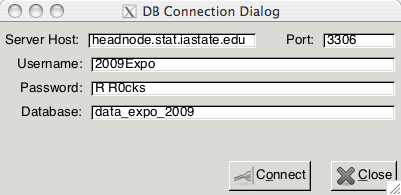
\includegraphics[width=3in]{dbconnect-dialog.png} 
   \caption{Dialog Window with connection information to the database. After clicking `Connect', the connection to the database is established.}
   \label{dbconnect}
\end{figure}
%\begin{center}
%\includegraphics[width=4in]{name.pdf}
%\end{center}


%\vspace{.5cm}

Selecting `Connect' establishes the connection to the database and opens up the main browser (Figures \ref{lineviewer} to \ref{dbquery}).  The main browser serves the following three main functions:
\begin{enumerate}
\item data display for easy and immediate verification of data entries, 
\item data retrieval/database sub-setting to prepare the data for subsequent statistical analysis, 
\item learning tool for the structured query language (SQL).
\end{enumerate}

The browser dialog consists of four tabs: the `Data Viewer,' the `Variable Browser,' the `Subsample' dialog, and a `Query' tab.  A list of the different data tables stored in the selected database is given in form of a (scrollable) second line of tabs underneath the main four tabs. Access to any of these data tables is obtained  by clicking on the corresponding data table tab; any functions of the browser dialog will now be applied to the selected data set. In our example, six data sets are stored in the database  providing information on flights, airports, planes, carriers, and weather conditions. 

%\textit{The first tab (displayed in Figure \ref{lineviewer}) is an introductory tab that provides the student with tips for working with the GUI. The tab also contains a list of frequently asked questions (FAQ) with answers that provide additional guidance to the students, such as, how to enter tail numbers, origin, destination, or flight numbers. Definitions for levels of categorical variables that are not self-explanatory (e.g., day of the week) are provided as well. The introductory tab also provides the student with an explanation of the interpretation in multiple selections. For example, if the student wants to research all cancellations of a specific aircraft, he/she will need to specify a tail number and set the checkmark for ``cancelled'' to yes. This extends an SQL statement by ``where TailNum in (' ') AND Cancelled=1.'' This tab can be easily adapted according to students' need and feedback.} \red{I don't recall this feature at all?? Did we do this indeed?}

The Data Viewer tab  (Figure \ref{lineviewer}) displays available information on the first five records of the selected data set (this is similar to the command {\tt head} in {\tt R}) providing an overview of the data and allowing students to familiarize with the available information.  

The variable browser (not shown) lists all the variables corresponding to the selected data set as well as the data type of the variables in both the SQL and S language.  


\begin{figure}[h] %  figure placement: here, top, bottom, or page
   \centering
   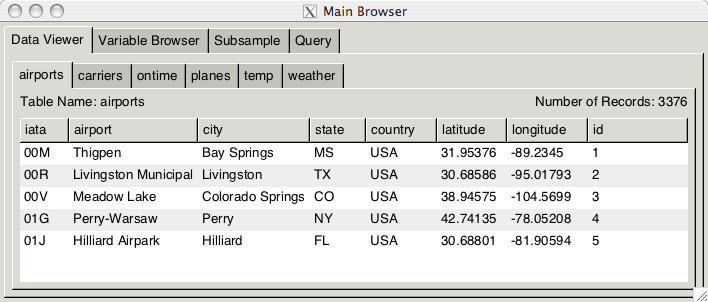
\includegraphics[width=4in]{db-lineviewer.png} 
   \caption{Data Viewer tab of the main browser dialog window. The line of tabs gives an overview of the available datasets. The first five records of the selected  dataset are shown.}
   \label{lineviewer}
\end{figure}

In the `Subsample' tab (see Figure \ref{dbsample}) the user can sequentially narrow the scope of the data set to a subset of interest by adding one variable criterium at a time. Criteria can be linked using either the `AND' or `OR' expression and any selection can be modified by removing the last specified criterium. The number of data records in the subsample can further be limited by setting a desired sample size  in the  `Limit' field. Specifying a limit will yield a selection of data records of the chosen size in the order the data records appear in the database. Alternatively, future development will extend this dialog to enable a (stratified) random selection of the records in the database.

Figure \ref{dbsample} shows a query from the `ontime' data set selecting the first 100 flights ({\tt{Limit:100}}) from 2008 ({\tt{Year=2008}}) during the month of January ({\tt{Month=1}}) that arrived in Chicago O'Hare airport ({\tt{Dest=ORD}}) with at least 15 minutes of delay ({\tt{ArrDelay>=15}}).  \\[.25cm]

\begin{figure}[htbp] %  figure placement: here, top, bottom, or page
   \centering
   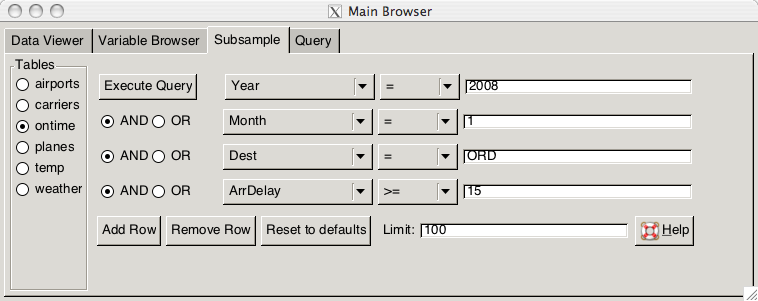
\includegraphics[width=4in]{db-sample.png} 
   \caption{Subsample tab of the main browser dialog window. Subsets of the data can be chosen using a sequence of logical expressions based on variable values. The SQL query corresponding to any sequence is shown in the Query Tab (see Figure \ref{dbquery}).}
   \label{dbsample}
\end{figure}

Upon choosing `Execute Query' the above selection of observations is automatically converted into the corresponding SQL statement yielding the following SQL query:

{\tt
\begin{tabular}{lllllr@{=\ }lllc}
 Select * from ontime where & ( & ( & ( & (& Year \  & 2008 &) && and \\
&&& &(& Month \ & 1 & ) & ) & and \\
&&& & (& Dest \ & 'ORD' & )& ) & and \\
&&& & (& ArrDelay > & 15& )& ) & limit 100
\end{tabular}
}

%\vspace{.25cm}
 
This SQL command will be displayed in the `Query' tab (shown in Figure~\ref{dbquery}). Logical expressions are connected sequentially using left-sided parentheses. Any later modifications to this structuring or extensions to the query in form of a more general SQL query, e.g. interconnecting several data tables, need to be made explicitly in the editable top section of the query tab (see Figure \ref{dbquery}).     \\[.25cm]
\begin{figure}[htbp] %  figure placement: here, top, bottom, or page
   \centering
   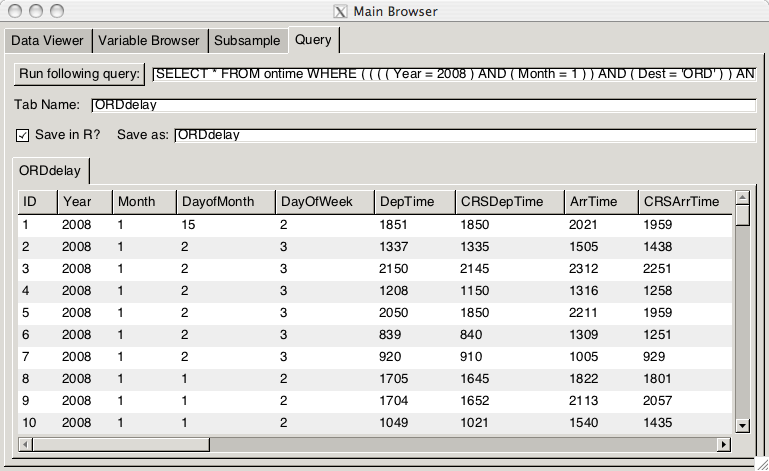
\includegraphics[width=4in]{db-query.png} 
   \caption{Query tab of the main browser dialog window. Once the SQL command is constructed (either manually or with the help of the subsample tab) the data records can be extracted from the database and imported into the {\tt R} session.}
   \label{dbquery}
\end{figure}


Once a query statement is specified in the `Query' tab and having checked the `Save in R' box, the corresponding data records can be extracted from the database and imported into the current {\tt R} session by submitting the `Run following query' button.  The retrieved data records will also be displayed in the `Query' tab (see Figure~\ref{dbquery}). \\
Prior submitting the query, the user can specify both a table name to distinguish data subsets if several different queries are run and a data file name in {\tt R}. In the example shown in Figure \ref{dbquery}, the data table name in the `Query' tab and the {\tt R} data file name is `ORDdelay.'
%
%
%
%\begin{figure}[htbp] %  figure placement: here, top, bottom, or page
%   \centering
%   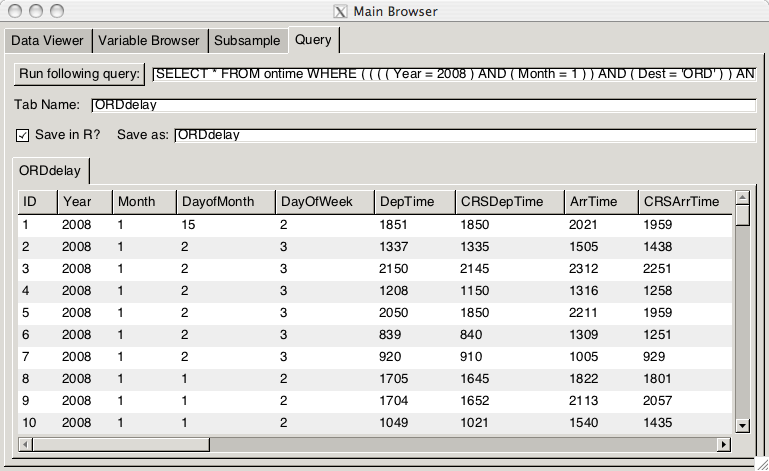
\includegraphics[width=4in]{db-query.png} 
%   \caption{Query tab of the main browser dialog window. Once the SQL command is constructed (either manually or with the help of the subsample tab) the data records can be extracted from the database and imported into the {\tt R} session.}
%   \label{dbquery-results}
%\end{figure}
%



\subsection{{Learning Objectives}}

%Need to consider the following questions:
%\begin{enumerate}
%\item What are the learning outcomes/goals we want to achieve with the GUI?
%\item How do we achieve them by using the GUI?
%\item Why does the GUI do a better job at achieving these learning outcomes than other tools (not sure what other tools are realistically available though)?
%\item Other benefits/uses for the GUI 
%\item Need to connect the main features of the GUI to pedagogical value, i.e. what is the purpose of a specific feature, what does it allow students to explore? 
%\end{enumerate}
%

The GUI facilitates multiple learning objectives: 

\begin{enumerate}
	\item Familiarizing students with databases and exploring the utility of databases for efficient data storage.
	\item Obtaining access to data stored in databases. 
	\item Searching databases for specific data records of interest as well as learning how to extract such data records for further statistical analysis in R or a different software package. 
	\item Providing students with a first gentle and more paced introduction to the SQL language. The GUI can help facilitate the learning process and potentially improve student's attitude toward learning the database language SQL.
\end{enumerate}	
 
All or a subset of these learning objectives can be selected by the instructor depending on the background of the students and the available classroom time.\\
Most students have no experience with databases (see student feedback section \ref{implement}) as at most universities and colleges the current training of students typically focuses on the use of statistical software packages such as SAS, JMP, Minitab or {\tt R}. All of these software packages are restricted to the use of data sets of manageable size. Furthermore, instructors tend to use data sets that are typically of small size consisting only of a few variables and a limited number of data records to optimally illustrate the statistical method under consideration.  Real-world data, however, is rarely available cleaned up this nicely and often tends to be much less tractable than data sets used in the classroom.   For this reason, we expect that in the majority of instances the primary learning objective will revolve around teaching students how to gain access to databases and how to subset data for further statistical analysis.

For the purpose of introducing students to the database language SQL, the `Subsample' and `Query' tab do provide students with the opportunity to explore the structure of SQL step by step at a pace that can be individually adjusted to the students' needs. In particular, students can receive immediate feedback upon modifying an existing SQL query: the generation of a data table confirms that students submitted a legitimate SQL query. Additionally, instructors can provide students with the final sample size of the desired data subset or subset related summary statistics to verify whether students submitted the correct SQL query.      


\section{Testing Usability of the GUI in the Classroom}
\label{implement}
In order to assess usability the GUI was tried out with students at Iowa State University, coming from two separate courses - one at the 400 level targeting Statistics undergraduates in their junior or senior year, the other one at the 500 level targeting Statistics graduate students in their freshman year. While the first course represents  our main audience, students from the second course represent an `after' audience - i.e. students who obviously have stayed in the field and have been recruited into our graduate program.  A small third group consisted of advanced graduate students seeking a degree outside statistics but having an interest in data analysis knowledge as their final degree.  Overall, 75 students participated in the usability survey; Table \ref{fb-overview} shows a summary of students by status, course, and main area of study. 

% Requires the booktabs if the memoir class is not being used
\begin{table}[htbp]
   \centering
   %\topcaption{Table captions are better up top} % requires the topcapt package
   \begin{tabular}{lrrrr} % Column formatting, @{} suppresses leading/trailing space
      \toprule
%      \cmidrule(r){1-2} % Partial rule. (r) trims the line a little bit on the right; (l) & (lr) also possible
	Course  & \multicolumn{2}{c}{400-level} & \multicolumn{2}{c}{500-level} \\
      \midrule
      & Statistics & non-Statistics       & Statistics & non-Statistics \\
       \cmidrule(l){2-5}
      Graduate & 1 & 8 & 21 & 15 \\
      Undergraduate & 23 & 6 & 1 & 0 \\
      \bottomrule
   \end{tabular}
   \caption{Overview of students participating in the usability study by course, status and area.}
   \label{fb-overview}
\end{table}

Students were initially surveyed about prior database knowledge. Results indicate that previous knowledge of database management systems differs between undergraduate and graduate students -- about 20\% of graduate students have had previous exposure to databases as opposed to just under 10\% of undergraduate students. There is no indication of any difference in exposure to databases between students majoring in statistics in comparison to students majoring in other disciplines. Students who had prior training in database systems had an average of 1.7 years of exposure. \\
Because the main purpose of the survey was to assess the ease of use of the GUI as an indicator of usefulness and functionality, students were not formally introduced to the GUI prior the survey. Instead students were given a set of instructions and GUI related questions to work through and to answer while using the GUI. Although this approach may appear somewhat extreme we felt that this would yield the most informative results with respect to the user-friendliness of the GUI.  The majority of questions asked in the survey is presented in Table \ref{fb-questions}. The table further shows marginal distributions of the correct answers by student status, i.e. graduate versus undergraduate students. (A complete list of all questions and the full survey is available at \url{http://heike.wufoo.com/forms/accessing-large-datasets/}.)

Questions were chosen such that students were led step by step through the different features of the GUI but at the same time allowing the assessment of student understanding. Questions focused on three different aspects: the understanding of the GUI and its main features, the understanding of the data, and the capability to impart some first SQL knowledge.  Two (graduate) students had difficulties with the interface to the extent that none of the data set and SQL related questions were answered correctly. Because these two students appeared to have struggled with the remaining course content as well, the lack of understanding, therefore, cannot be attributed exclusively to the GUI set-up. For questions regarding SQL commands (questions 9 - 11, see Table \ref{fb-questions}), 64 students were able to correctly answer question \#9, 37 correctly answered question \#10, and 39 students correctly answered question \#11. A careful analysis of false answers submitted by students revealed that some of the erroneous answers were likely due to carelessness rather than lack of understanding. In particular, Figure \ref{fb-errors} provides more detailed information on the type of mistakes made by students and summarizes errors by error sources, e.g. for question \#10 wrong use of logical expressions in the `Subsample' tab, failure to use the correct variable name, and mis-specified text values were leading causes of errors (the category `value' indicates mis-specified variable names or values while the category `logic' indicates wrong use of logical expressions).  

\begin{figure}[htbp] %  figure placement: here, top, bottom, or page
   \centering
   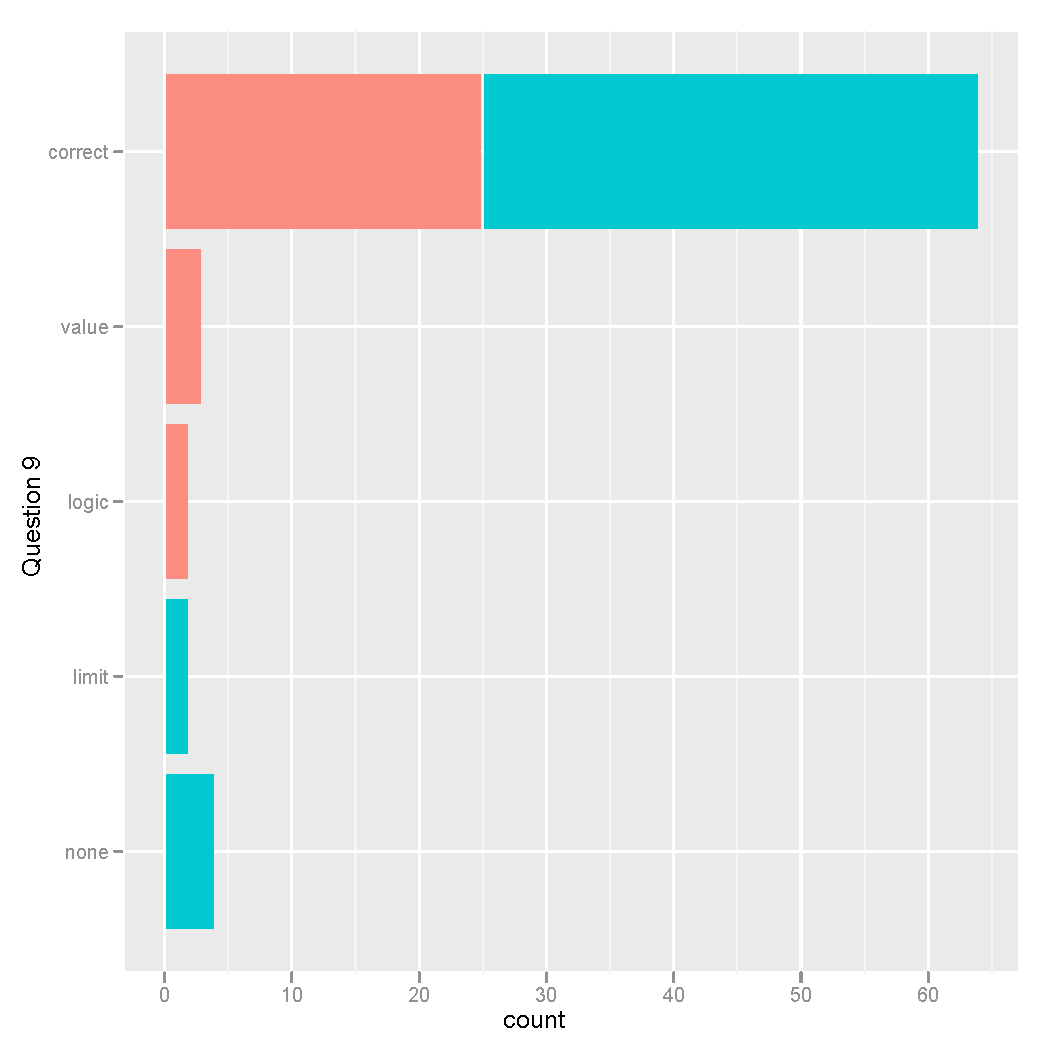
\includegraphics[height=2in,  keepaspectratio=true]{fb-question-9.pdf} 
   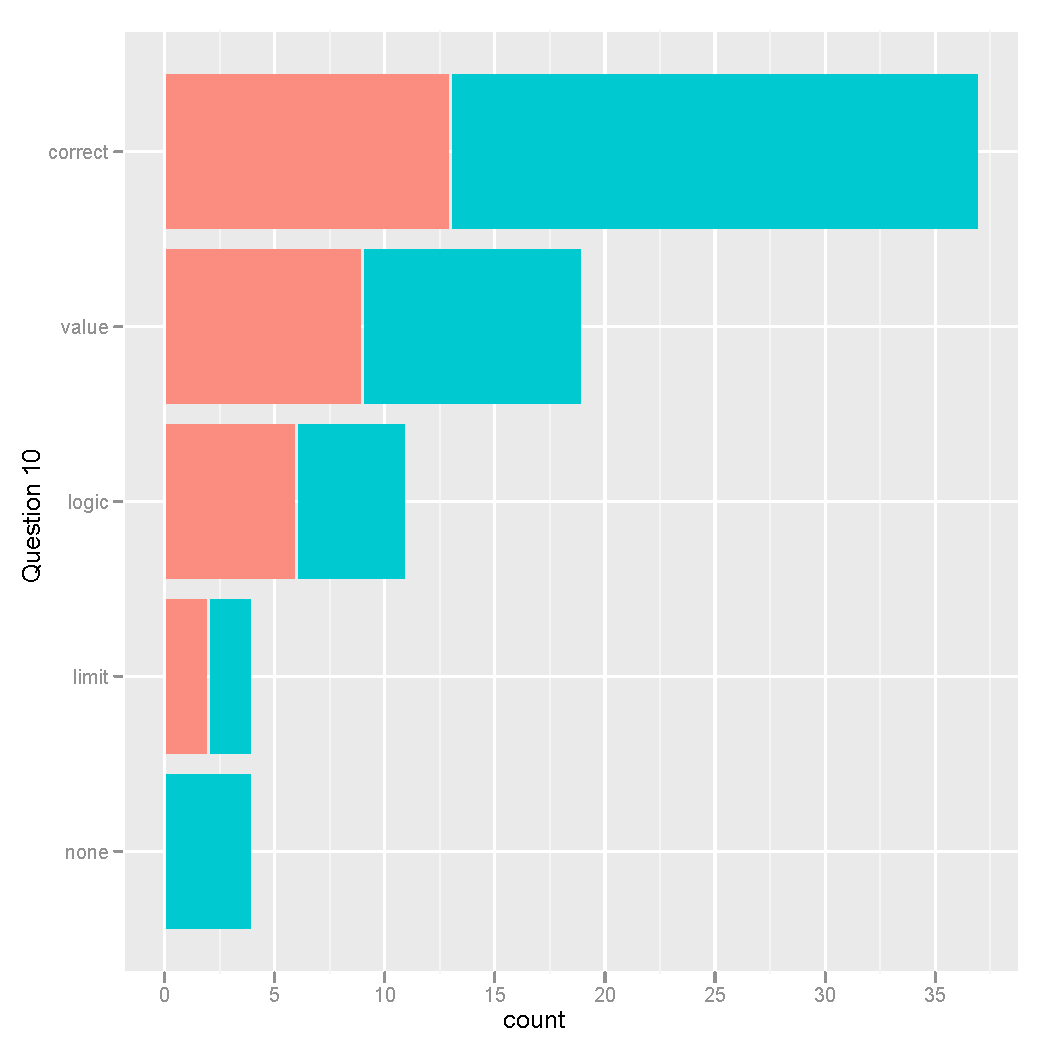
\includegraphics[height=2in,  keepaspectratio=true]{fb-question-10.pdf} 
   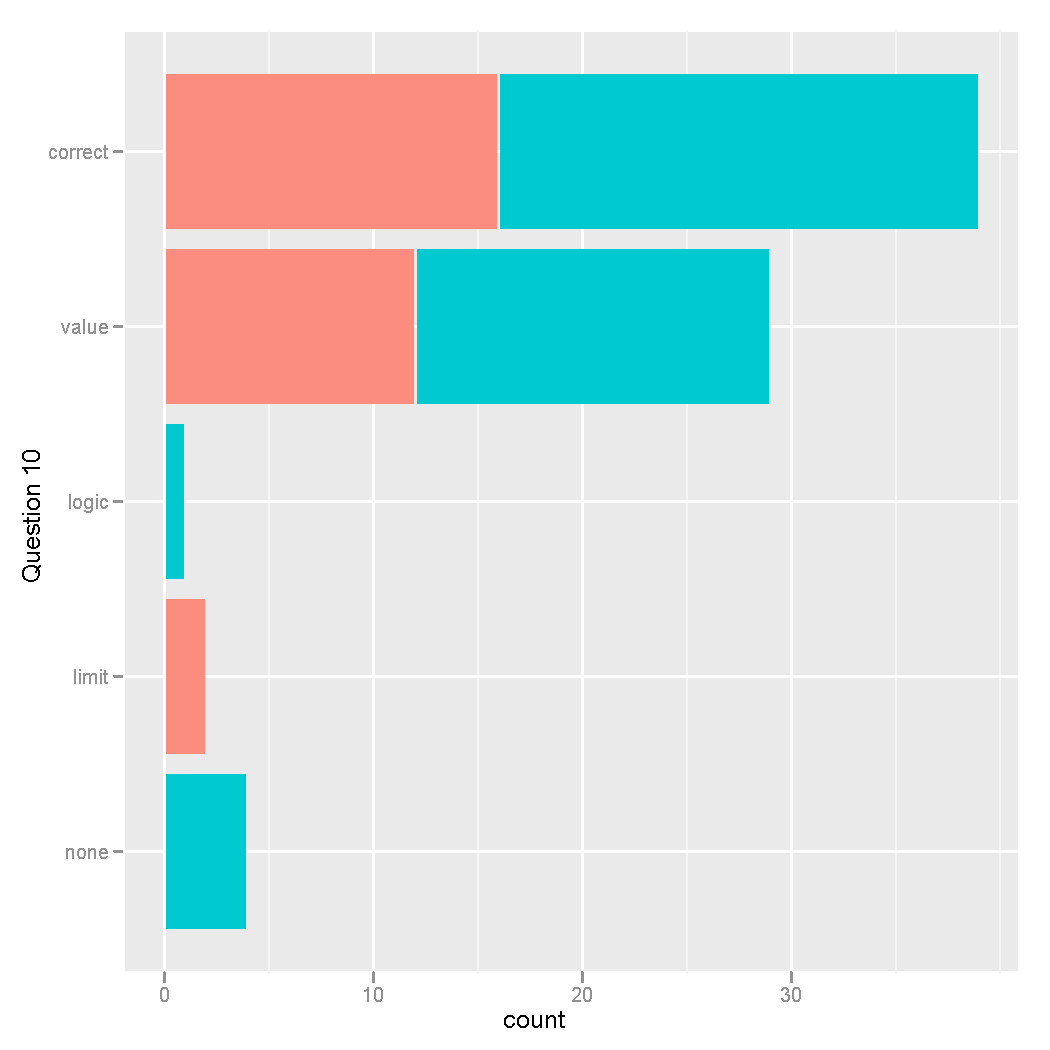
\includegraphics[height=2in,  keepaspectratio=true]{fb-question-11.pdf} 
 
   
\includegraphics[height=.25in, keepaspectratio=true]{fb-legend2.pdf} 
   \caption{Students' feedback on questions 9, 10, and 11. Wrong answers are classified according to source of error. `value' and `logic' can potentially be considered carelessness errors rather than mistakes due to lack of understanding of the GUI. Categories `limit' (specifying a wrong limit of data records) and `none' (not providing any answer) are more serious errors and indicate a lack of understanding of the GUI.} %(for question \#11 $\le$ and $<$, and $\ge$ and $>$ were no longer distinguished).}
   \label{fb-errors}
\end{figure}

Figure \ref{fb-use-importance} shows results regarding the perceived importance of the task and how useful students felt the GUI was in completing the task. Although graduate students show a more clear understanding of the importance of database knowledge as compared to the undergraduate students, both groups 
respond similarly about the GUI's usefulness to complete the task.

\begin{figure}[htbp] %  figure placement: here, top, bottom, or page
   \centering
   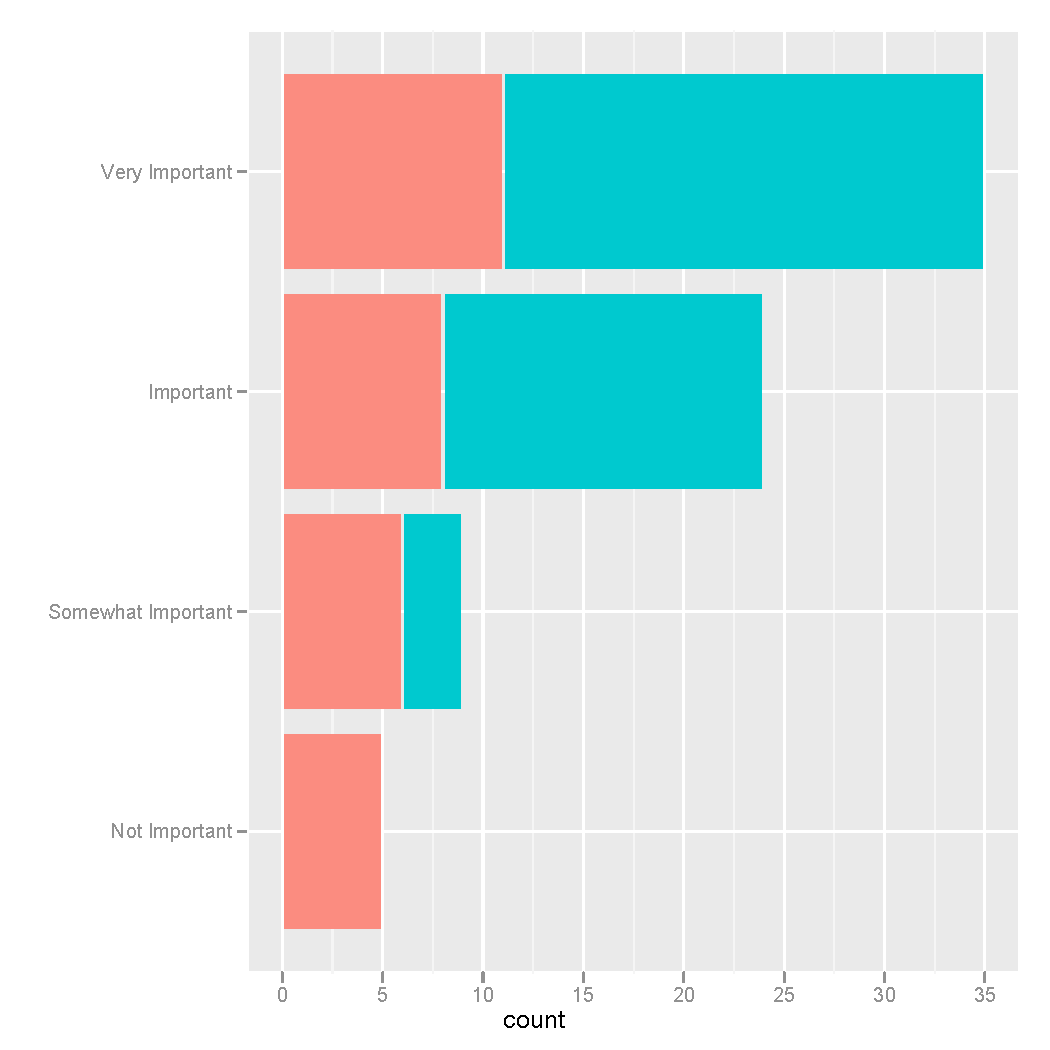
\includegraphics[height=2in, keepaspectratio=true]{fb-importance.pdf} 
   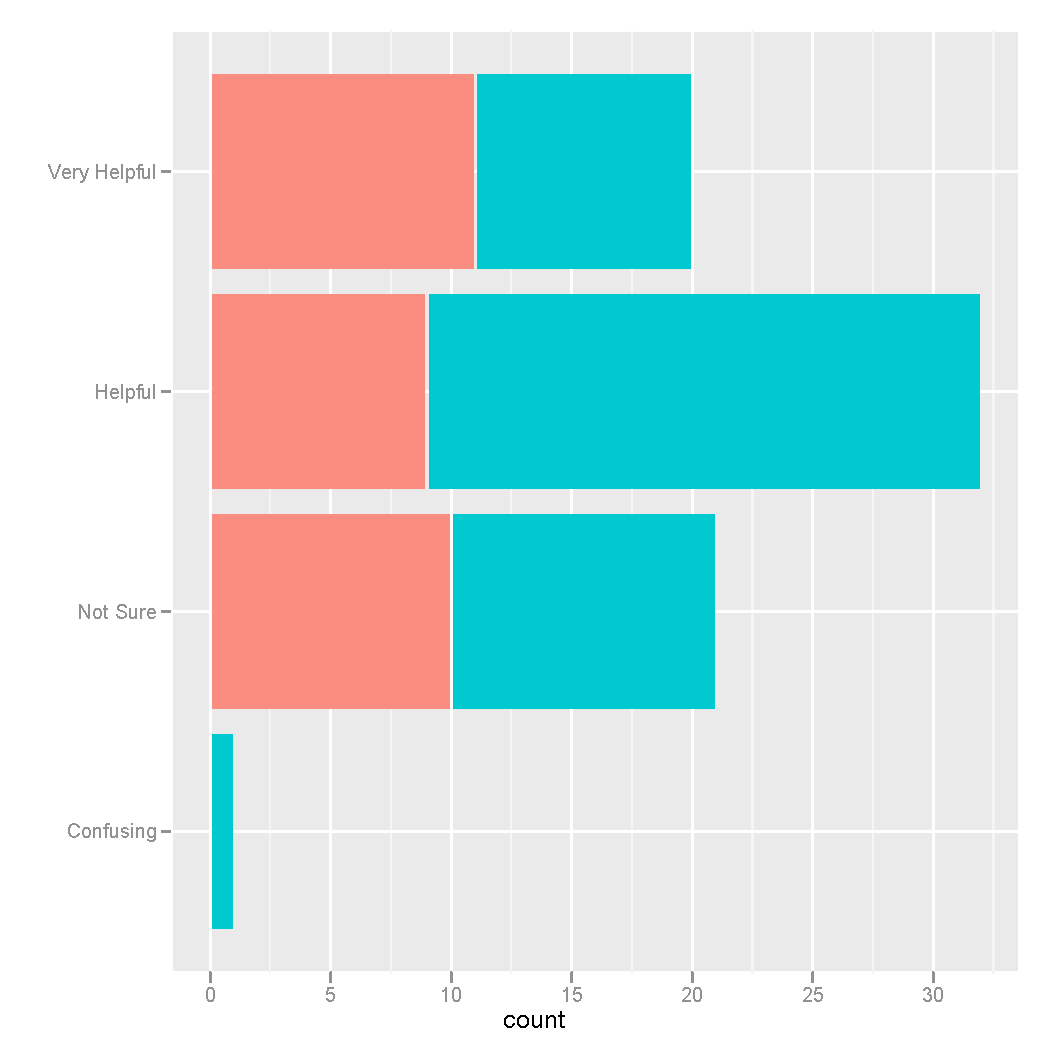
\includegraphics[height=2in, keepaspectratio=true]{fb-useful.pdf} 
   
\includegraphics[height=2in, keepaspectratio=true]{fb-legend.pdf} 
   \caption{User feedback: perceived importance of task (left) and usefulness of the GUI to help with the task (right).}
   \label{fb-use-importance}
\end{figure}

Figures \ref{fb-before-after} and \ref{fb-before-and-after} illustrate that the GUI successfully facilitated the completion of the task. The task difficulty was clearly perceived higher by students before the use of the GUI than afterwards. Figure \ref{fb-before-after} shows marginal distribution of assessed class difficulty, while the fluctuation diagram of figure \ref{fb-before-and-after} shows the joint distribution. Very few students  find the task harder than anticipated - we take this as an indicator that the GUI is a useful resource for introducing students to databases as intended.  


\begin{figure}[htbp] %  figure placement: here, top, bottom, or page
   \centering
Students' assessment of task difficulty 

   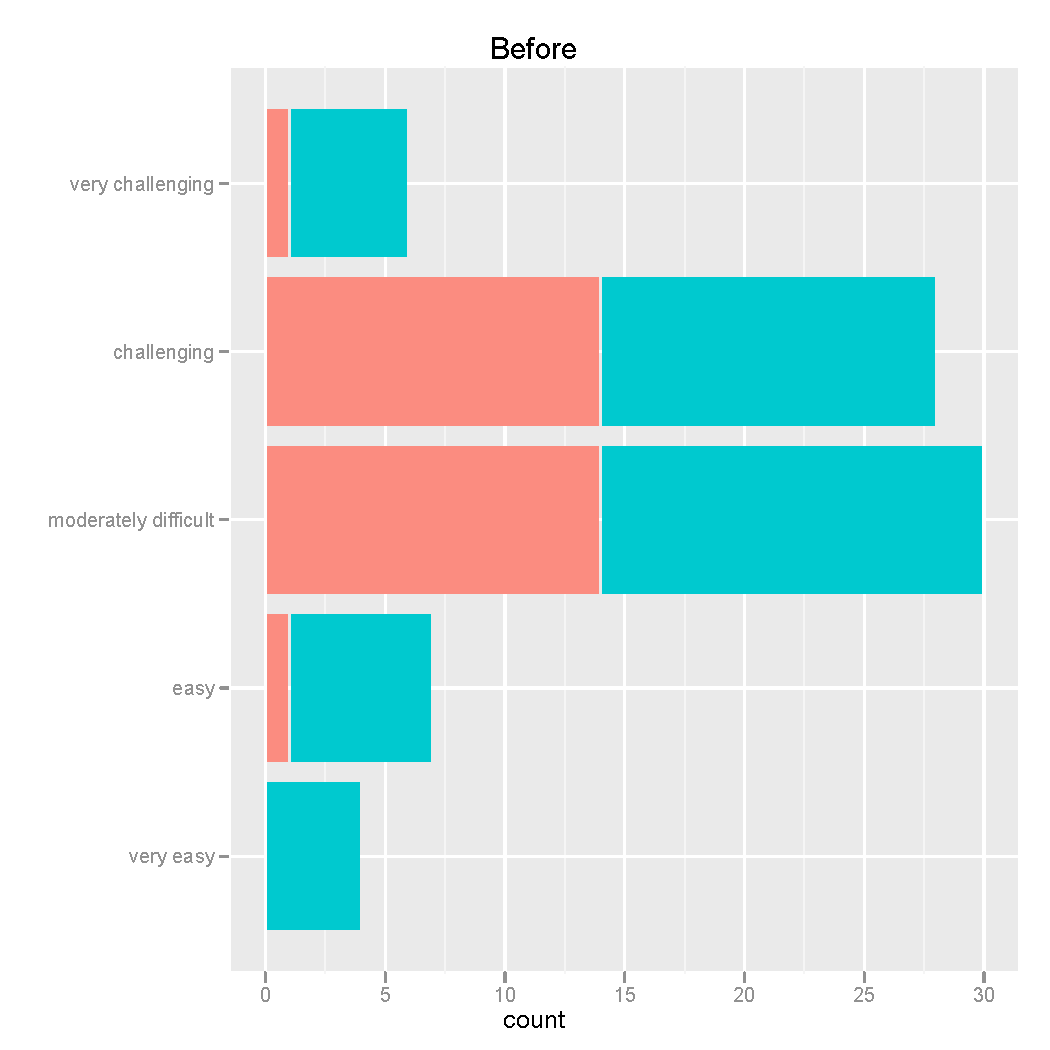
\includegraphics[height=2in,  keepaspectratio=true]{fb-before.pdf} 
   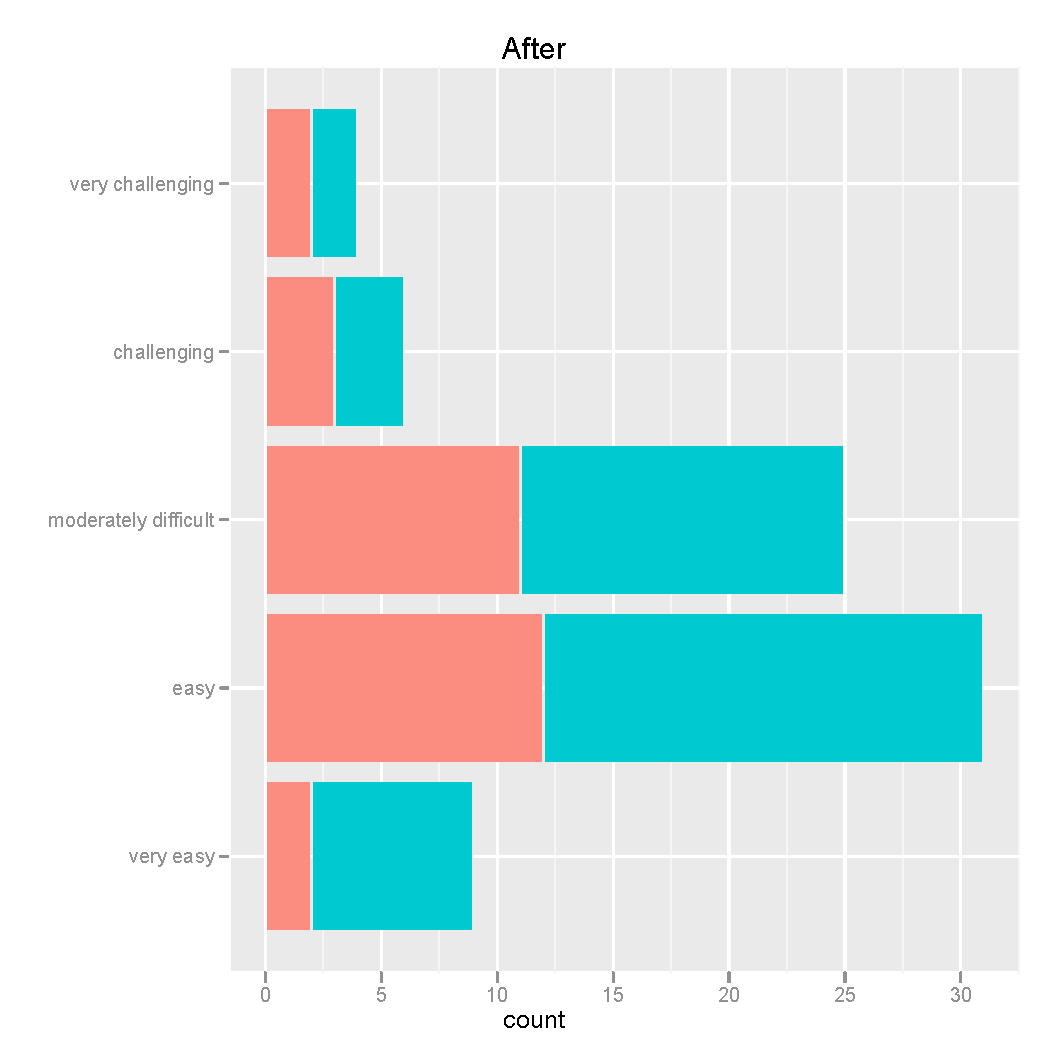
\includegraphics[height=2in,  keepaspectratio=true]{fb-after.pdf} 
   
\includegraphics[height=2in,  keepaspectratio=true]{fb-legend.pdf} 
   \caption{User feedback: anticipated degree of difficulty is greater than experienced difficulty of the task.}
   \label{fb-before-after}
\end{figure}

%\vspace{2cm}


\begin{figure}[htbp] %  figure placement: here, top, bottom, or page
   \centering
   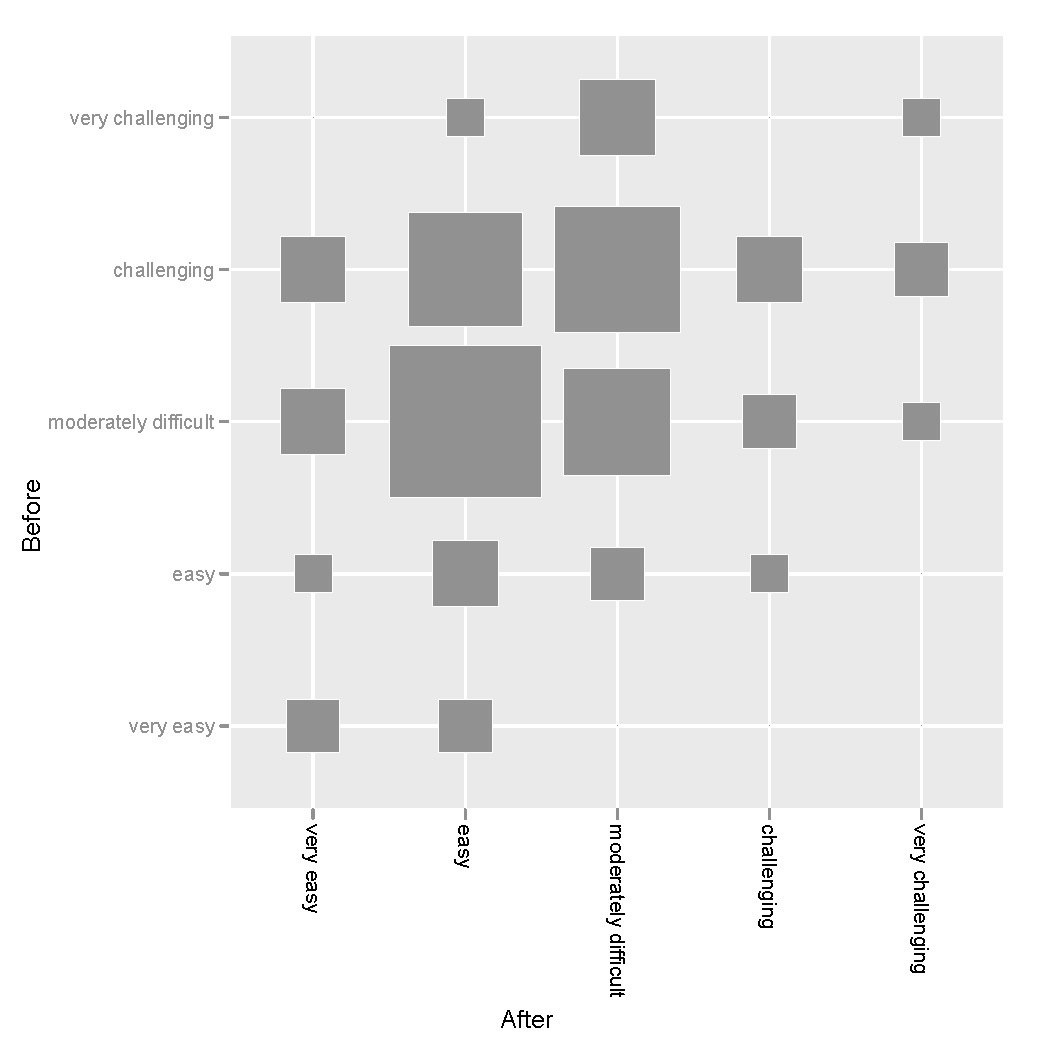
\includegraphics[height=3in, keepaspectratio=true]{fb-before-after.pdf} 
   \caption{Fluctuation diagram of students' assessment of task difficulty before and after completion of  the study. Generally, students find the task easier than they anticipate.}
   \label{fb-before-and-after}
\end{figure}




\begin{table}[htbp]
   \centering
   %\topcaption{Table captions are better up top} % requires the topcapt package
   \begin{tabular}{p{4.5in}rr} % Column formatting, @{} suppresses leading/trailing space
      \toprule
%      \cmidrule(r){1-2} % Partial rule. (r) trims the line a little bit on the right; (l) & (lr) also possible
	\textbf{Question}  & \multicolumn{2}{l}{\textbf{Correct Answers} (\%)} \\
      \cmidrule{2-3}
 & U'grad. & Grad. \\ 
  \cmidrule(l){1-3}
\multicolumn{3}{l}{\textbf{Questions regarding the Interface}}\\
  \cmidrule(l){1-3}
  \footnotesize
1. Upon opening the GUI, you should see two lines of tabs.  What is the default tab opened in row 1, what is the default in row 2? & \footnotesize 100.0 & \footnotesize 95.6 \\ 
\footnotesize 2. List the first two airports and cities (case records) that are displayed.  & \footnotesize 100.0 & \footnotesize 95.6 \\ 
\footnotesize 3. How many rows of case records are displayed by default when opening the GUI?  & \footnotesize 96.7 & \footnotesize 84.4 \\ 
  \cmidrule(l){1-3}
\multicolumn{3}{l}{\textbf{Questions assessing basic understanding}}\\
  \cmidrule(l){1-3}
\footnotesize 4. Does the dataset contain more case records than the ones displayed? & \footnotesize 93.3 & \footnotesize 93.3 \\ 
\footnotesize 5. The ontime tab contains all the flight information. What is the total number of flights in the database?  & \footnotesize 80.0 & \footnotesize 91.1 \\ 
\footnotesize 6. Which data table has the fewest variables?  & \footnotesize 100.0 & \footnotesize 95.6 \\ 
\footnotesize 7. Which data table has the most variables (don't count, just eyeball)? & \footnotesize 93.3 & \footnotesize 95.6 \\ 
  \cmidrule(l){1-3}
\multicolumn{3}{l}{\textbf{Advanced questions: questions assessing SQL understanding}}\\
  \cmidrule(l){1-3}
\footnotesize 9. Select the `ontime' radio button. This data set contains information on all commercial flights over the last 20+ years. Specify to select a limit of 100 flights in 2001. Once you're done, press `Execute Query'. The GUI will change to a view (the Query tab), where you can see the resulting query. Copy the query and paste it into the space below: & \footnotesize 83.3 & \footnotesize 86.7 \\
\footnotesize 10. Change back to the `Subsample' tab.  Change your sample. Remove the limit, but now only select flights into Des Moines (DSM), that were delayed by at least 60 minutes on arrival - the year is still 2001.  Again, execute the query and paste the resulting SQL statement into the space below: & \footnotesize 43.3 & \footnotesize 53.3 \\
\footnotesize 11. Without the help of the GUI change the SQL statement from question 10 such that you only regard flights that were not delayed upon departure (less than 15 min delayed).  Paste the resulting query into the space below: & \footnotesize 53.3 & \footnotesize 51.1 \\ 
      \bottomrule
   \end{tabular}
   \caption{Questions of the usability study, marginal distribution of correctly answered questions.}
   \label{fb-questions}
\end{table}
\label{implement}
%\begin{enumerate}
%\item talk about 480 and 579
%\end{enumerate}
%

%Figure \ref{dbquery} shows the type-dependent summary of all variables: the minimum and maximum value for numerical variables and the list of levels for a categorical variable. This information enables the student to screen the database for invalid data entries (e.g., negative minimal values for the actual elapsed time of an airplane between leaving the gate at the originating airport and arriving at the destination airport gate that can theoretically only be positive; see Figure \ref{dbquery}). The student immediately gets prompted to further investigate the data before beginning with any statistical analyses that potentially might lead to erroneous results.
%The last tab of the main browser (Figure 4) allows the student to retrieve data from the database and to import it as regular data frames into R. Samples can be taken from the entire database or just from a range of data values/variable levels by specifying the lower and upper endpoints in editable text boxes in the previous tabs (Figure 3). Samples sizes are determined according to the sampling fraction of interest and taken at random from the chosen portion of the database.
%The GUI serves also as a learning tool for the SQL as it provides textual output of the session's SQL commands that then can be saved for future reference by the students. This helps students to overcome an often steep and intimidating initial learning curve.
%\begin{center}
%screenshot
%\end{center}



%\newpage

\section{{Dissemination and Developmental Outlook}}
To achieve a broad dissemination of the developed GUI, the database is accessible for public use and stored on a server of the Department of Statistics at Iowa State University. An accompanying webpage is available at \url{http://www.public.iastate.edu/~hofmann/vldb.html}.
This webpage provides the following information and tools: 
\begin{enumerate} 
\item a link to the {\tt R} source code for the GUI - also available in form of the {\tt R} package {\tt dbConnector} available on CRAN, 
\item information on accessing the SQL database for the `09 ASA Data Expo, 
\item a detailed description of the data,  
\item examples and sample analyses for classroom demonstration, 
\item a growing list of links to other databases accessible on the server at Iowa State University, 
\item contact information for feedback.
\end{enumerate}
In particular, we seek to implement more of the SQL functionality into the graphical user interface. While the query tab allows the full spectrum of the Select Query Language, we have only implemented the interface to data sub-setting. We are preparing to also support a user interface for joining data across several tables, and allowing stratified sampling. 
Other databases that are currently available from the server at Iowa State University include information on how and where money made available through the American Recovery and Reinvestment Act 2009 (ARRA) is being spent. This is data made publicly available by \url{recovery.gov}, which was being used in \citet{designforamerica}'s `Design for America' Challenge. More information about the data is available through \citet{arra}.
%As mentioned earlier, current development is underway that will allow random sampling from the database (\red{Dason or Heike, can you add a sentence explaining the technical challenge associated with this task?}). 
Once the GUI also supports random sampling, it can also be used as a data resource for instructors allowing, for example, to sample data sets individually for classes or students that will yield different numerical results in a statistical analysis without changing the context of the data or task, while at the same time allowing for an automatic assessment of correctness of answers.    

We introduced the idea of a graphical user interface that allows an introduction of data sets into classroom that otherwise are too large in size to be managed by commonly used statistical software. We explained some of the technical and pedagogical aspects of the GUI and an extension of the GUI is currently under development. Although the GUI has been used successfully in the classroom a full implementation and evaluation of the GUI is still necessary and currently being prepared.

%\newpage
\bibliography{references}
\end{document}












